\chapter{Aprendizado supervisionado}
\label{cap:aprendizado-supervisionado}

\framebox[\textwidth]{
	\hspace{1em}
	\vbox{
		\textbf{Leitura obrigatória:}
		\begin{itemize}
			\item \cite{FaceliEtAl2011} -- Cap. 4 (Métodos Baseados em Distâncias).
			\item \cite{Mitchell1997} -- Cap. 3 (Decision Tree Learning).
		\end{itemize}
		
		\textbf{Leitura complementar:}
		\begin{itemize}
			\item \cite{RusselAndNorvig2010} -- Cap. 18 (Aprendendo através de exemplos).
			\item \cite{MullerAndGuido2017} -- Cap. 2 (Supervised Learning).
		\end{itemize}
	}
}

\section{Visão geral}

Conforme discutido no Capítulo~\ref{cap:conceitos-basicos-aprendizagem-maquina}, o aprendizado supervisionado é aplicado a tarefas preditivas de classificação e regressão. As técnicas de aprendizado supervisionado se baseiam em um conjunto de dados rotulados e tem por objetivo aprender uma hipótese ou função que relacione os atributos de entrada com o atributo de saída. Com isso, o valor do atributo de saída de uma nova entrada pode ser estimada.

A aprendizagem é chamada supervisionada pois os dados servem como exemplos, que são utilizados durante o processo de aprendizagem. Com isso, cada tentativa de predição é avaliada por um ``supervisor'', o qual se baseia nos dados rotulados. Este paradigma exige um esforço humano em rotular um conjunto de dados para a aprendizagem, mas produzem hipóteses que podem ser utilizadas em tarefas de predição futuras. Os dados rotulados utilizados na indução da hipótese são chamados de \textbf{conjunto de treinamento}, enquanto os dados utilizados para validar a hipótese induzida são chamados de \textbf{conjunto de teste}. O processo de aprendizagem, portanto, pode ser chamado de \textbf{treinamento} do modelo.

Após realizado o treinamento do modelo, temos um \textbf{estimador}, capaz de predizer o valor do atributo alvo de novos e desconhecidos dados. Caso o atributo alvo toma valores de um domínio de valores nominais, temos a tarefa de \textbf{classificação} e chamamos o modelo de \textbf{classificador}. Caso o atributo alvo toma valores em um intervalo contínuo e ordenado, temos uma tarefa de \textbf{regressão} e chamamos o modelo de \textbf{regressor}.

A Tabela~\ref{tab:exemplo-classificacao} apresenta um exemplo de classificação. Trata-se de parte do conjunto de dados chamado \texttt{iris}, que contém registros do tamanho (comprimento e largura) da pétala e da sépala de diferentes flores íris. Com base nos quatro atributos de entrada, a tarefa consiste em classificar as flores segundo sua espécie: íris setosa, íris versicolor ou íris virgínica. Perceba que o atributo alvo (espécie) consiste em um valor nominal (conjunto discreto) e, portanto, trata-se de uma tarefa de classificação.

\begin{table}[h]
	\centering
	
	\begin{tabular}{rrrrl}
		\hline
		\textbf{Comp. (P)} & \textbf{Larg. (P)} & \textbf{Comp. (S)} & \textbf{Larg. (S)} & \textbf{Espécie} \\
		\hline
		5,1 & 3,5 & 1,4 & 0,2 & Setosa \\
		4,9 & 3,0 & 1,4 & 0,2 & Setosa \\
		7,0 & 3,2 & 4,7 & 1,4 & Versicolor \\
		6,4 & 3,2 & 4,5 & 1,5 & Versicolor \\
		6,3 & 3,3 & 6,0 & 2,5 & Virgínica \\
		5,8 & 2,7 & 5,1 & 1,9 & Virgínica \\
		$\vdots$ & $\vdots$ & $\vdots$ & $\vdots$ & $\vdots$ \\
		\hline
	\end{tabular}
	
	\caption{Exemplo de classificação das espécies de íris}
	\label{tab:exemplo-classificacao}
\end{table}

A Tabela~\ref{tab:exemplo-regressao} apresenta um exemplo de regressão. Trata-se de um conjunto de dados chamado \texttt{swiss}, que contém registros estatísticos de uma população, como educação e taxa de fertilidade. A tarefa é definir, com base nos atributos de entrada, a taxa de mortalidade da população (atributo alvo). Trata-se de um problema de regressão, pois o atributo alvo pode assumir qualquer valor em um intervalo contínuo.

\begin{table}[h]
	\centering
	
	\begin{tabular}{rrrrr}
		\hline
		\textbf{Fertilidade} & \textbf{Agricultura} & \textbf{Educação} & \textbf{Renda} & \textbf{Mortalidade} \\
		\hline
		80,2 & 17,0 & 12 & 9,9 & 22,2\\
		83,1 & 45,1 & 9 & 84,8 & 22,2\\
		92,5 & 39,7 & 5 & 93,4 & 20,2\\
		85,8 & 36,5 & 7 & 33,7 & 20,3\\
		76,9 & 43,5 & 15 & 5,2 & 20,6\\
		$\vdots$ & $\vdots$ & $\vdots$ & $\vdots$ & $\vdots$ \\
		\hline
	\end{tabular}
	
	\caption{Exemplo de regressão da taxa de mortalidade}
	\label{tab:exemplo-regressao}
\end{table}

Finalmente, a Figura~\ref{fig:exemplo-classificacao-regressao} ilustra as tarefas de classificação e regressão. Na primeira imagem, a classe do objeto é determinada em função dos valores das duas características de entrada, que são representadas pelos eixos $x$ e $y$. Na segunda imagem, o eixo $x$ apresenta o valor de uma característica, enquanto o eixo $y$ mostra o valor do atributo alvo. A tarefa consiste em determina a função que mapeia o valor no atributo de entrada para o valor do atributo alvo.

\begin{figure}[h]
	\centering
	\includegraphics[width=\textwidth]{img/exemplo-classificacao-regressao}
	\caption{Ilustração das tarefas de classificação e regressão}
	\label{fig:exemplo-classificacao-regressao}
\end{figure}

\section{Algoritmo \textit{k}NN -- \textit{k}-Nearest Neighbors}

O algoritmo do $k$NN (do inglês $k$-Nearest Neighbors), ou $k$-Vizinhos Mais Próximos é um método de aprendizagem de máquina baseado em instância, também classificado por muitos autores como uma técnica de \textbf{raciocínio baseado em casos}. O $k$NN considera a proximidade dos dados (das instâncias) para realização da predição. Ele consiste na técnica mais simples de aprendizagem de máquina e pode ser aplicado tanto para classificação como para regressão. A ideia principal é de que \textit{objetos relacionados ao mesmo conceito são semelhantes entre si}. O $k$NN é uma técnica simples pois não aprende um modelo compacto para os dados, mas memoriza todos eles durante a fase de treinamento, para então classificar novos dados com base na proximidade dos existentes.

\subsection{Esquema geral}

A distância entre dois objetos pode ser determinada pela distância euclidiana, calculada com base nos valores dos seus atributos de entrada. Seja $x_i$ o valor do atributo $i$ do objeto $x$ e $d$ o número de atributos do objeto, a distância entre dois objetos $a$ e $b$ pode ser definida como:
$$
d(a, b) = \sqrt{\sum_{i=1}^{d} (a_i - b_i)^2}
$$

\textbf{Observações:}
\begin{itemize}
	\item Esta medida é chamada de \textbf{distância euclidiana}. Existem outras medidas que podem ser aplicadas, como a \textit{distância de Manhattan} ou a \textit{distância Supremum}.
	\item Caso o atributo $i$ seja qualitativo (nominal, por exemplo), $a_i - b_i = 1$, caso $a_i \neq b_i$ e 0, caso contrário. Neste caso, é comum eliminar a radiciação do cálculo da distância.
	\item Existem outras medidas de distância para atributos qualitativos, como a \textit{separação angular} e a \textit{correlação de pearson}.
\end{itemize}

\insertspace

O algoritmo kNN estima o valor do atributo alvo de um novo objeto com base nos seus $k$ vizinhos mais próximos. Ou seja, dado um novo objeto, o algoritmo calcula a distância entre si e cada objeto do conjunto de treinamento, selecionando os $k$ mais próximos. No caso da classificação, o algoritmo atribui ao novo objeto a classe destes vizinhos. Caso ocorra divergências, o algoritmo seleciona a classe mais frequente, chamada de classe majoritária. Esta estratégia é chamada de \textbf{votação}. No caso da regressão, o algoritmo calcula a média dos valores dos $k$ vizinhos mais próximos, ou ainda outra medida estatística (como a mediana, por exemplo).

O caso mais simples é o algoritmo 1NN, que considera apenas o vizinho mais próximo e seleciona sua classe para a predição (ou o valor numérico do seu atributo alvo). A Figura~\ref{fig:exemplo-1nn} mostra um conjunto de dados onde os dados de treinamento são apresentados como círculos em azul (para a classe 0) e triângulos em vermelho (para a classe 1). Os dados de teste são apresentados como estrelas e sua cor indica a classe que foi atribuída a cada um. Como podemos perceber, a classe do vizinho mais próximo é atribuída ao novo dado.

\begin{figure}[h]
	\centering
	\includegraphics[width=0.7\textwidth]{img/exemplo-1nn}
	\caption{Exemplo de aplicação do algoritmo 1NN}
	\label{fig:exemplo-1nn}
\end{figure}

\begin{figure}[h]
	\centering
	\includegraphics[width=0.7\textwidth]{img/exemplo-3nn}
	\caption{Exemplo de aplicação do algoritmo 3NN}
	\label{fig:exemplo-3nn}
\end{figure}

Ao executar o algoritmo com um número maior de vizinhos, a predição torna-se mais precisa. A Figura~\ref{fig:exemplo-3nn} mostra o mesmo conjunto de dados sendo utilizado para a predição de três novos dados usando o algoritmo de 3NN. Neste caso, a classe é atribuída conforme os 3 vizinhos mais próximos, utilizando a estratégia de votação para resolver divergências. Perceba que a estrela do canto superior esquerdo, apesar de estar mais próxima a um objeto da classe 0, possui maior similaridade com a classe 1, pois a região superior é dominada por objetos desta classe. Esta característica só foi identificada com o uso de um maior número de vizinhos. Por outro lado, deve-se tomar cuidado para não atribuir um número muito elevado de vizinhos, gerando sub e sobreajuste. Cabe ressaltar que em tarefas de classificação binária, onde existem apenas duas classes possíveis, um número ímpar de vizinhos deve ser utilizado para evitar empates.

A Figura~\ref{fig:exemplo-1nn-regressao} mostra a aplicação do algoritmo 1NN para uma tarefa de regressão. O eixo $x$ mostra a característica, enquanto o eixo $y$ mapeia o valor do atributo alvo. O valor da predição é igual ao vizinho mais próximo do dado a ser estimado. A Figura~\ref{fig:exemplo-3nn-regressao} mostra a mesma tarefa sendo executada por um algoritmo 3NN. Dado o maior número de vizinhos, o valor alvo é melhor estimado, como pode ser percebido no primeiro dado de teste (mais a esquerda).

\begin{figure}[h]
	\centering
	\includegraphics[width=0.85\textwidth]{img/exemplo-1nn-regressao}
	\caption{Exemplo de aplicação do algoritmo 1NN para regressão}
	\label{fig:exemplo-1nn-regressao}
\end{figure}

\begin{figure}[h!]
	\centering
	\includegraphics[width=0.85\textwidth]{img/exemplo-3nn-regressao}
	\caption{Exemplo de aplicação do algoritmo 3NN para regressão}
	\label{fig:exemplo-3nn-regressao}
\end{figure}

A medida de similaridade dos objetos é impactada pela ordem de grandeza dos atributos de entrada. Considere um atributo $x$ que assume um valor no intervalo $[1, 10]$, e um segundo atributo $y$ que assume um valor no intervalo $[1, 1000]$. Agora considere que um objeto possui os seguintes valores de atributos $(x, y) = (1, 1)$. Se definirmos um segundo objeto com valores $(10, 10)$, temos que este objeto é muito distante do primeiro ao considerar o atributo $x$, mas bastante próximo ao considerar o atributo $y$. No entanto, a diferença absoluta entre os valores dos atributos de cada objeto é a mesma (10). Ou seja, o valor 10 significa distância máxima com relação ao atributo $x$, e proximidade com relação ao atributo $y$. Ao considerar apenas valores absolutos, o método pode induzir uma hipótese de baixa qualidade por conta da sensibilidade em relação à ordem de grandeza de diferentes atributos. Por isso, é recomendável que todos os atributos quantitativos passem por um processo de \textbf{normalização} antes de executar o algoritmo $k$NN.

A normalização pode ser feita selecionando, a partir dos dados de treinamento, o maior valor apresentado. Este valor passa a ser 1 e todos os demais são atualizados proporcionalmente. Por exemplo, se o maior valor de um atributo é 100, este passa a valer 1 e o valor 75 passa a valer 0,75, e assim por diante. Com isso, todos os atributos quantitativos terão intervalo $[0, 1]$, resolvendo o problema da sensibilidade à grandeza dos atributos.

\textbf{Observação:} além da normalização, outra medida de pré-processamento recomendada é a eliminação de atributos irrelevantes. Por exemplo, para definir se o paciente é \textit{doente} ou \textit{saudável}, não importa saber o valor do atributo \texttt{nome}.

\subsection{Análise do algoritmo}

Para um algoritmo $k$NN, podemos definir as áreas do conjunto de dados que resultarão na predição de cada classe. Isto é, se um novo dado se encontrar em uma determinada área, ele receberá a classe correspondente. A Figura~\ref{fig:analise-knn} mostra as áreas para as classes 0 e 1 para diferentes valores de $k$. Como pode ser observado, a predição com 9 vizinhos divide o conjunto de dados utilizando uma fronteira de decisão mais simples e, por isso, possui uma melhor generalização.

\begin{figure}[h]
	\centering
	\includegraphics[width=\textwidth]{img/analise-knn}
	\caption{Análise do algoritmo KNN para classificação com diferentes valores de $k$}
	\label{fig:analise-knn}
\end{figure}

A mesma ideia se aplica para problemas de regressão. A Figura~\ref{fig:analise-knn-regressao} mostra a execução do algoritmo com diferentes valores de vizinhos. Ao utilizar apenas 1 vizinho, a predição se ajusta aos dados de treinamento. O \textit{score} de treinamento é 1,00, enquanto o \textit{score} do teste é baixo (0,35). Ao aumentar o número de vizinhos, o \textit{score} de treinamento diminui, pois o modelo deixa de se ajustar perfeitamente aos dados de treinamento, mas aumenta a capacidade de generalização, o que é percebido no crescimento do \textit{score} de teste. Em outras palavras, com um maior número de vizinhos a predição produz uma curva que não possui predição exata para os dados de treinamento, mas generaliza melhor para novos dados.

\begin{figure}[h]
	\centering
	\includegraphics[width=\textwidth]{img/analise-knn-regressao}
	\caption{Análise do algoritmo KNN para regressão com diferentes valores de $k$}
	\label{fig:analise-knn-regressao}
\end{figure}

Apesar dessas análises indicarem problemas ao se utilizar um número muito baixo de vizinhos, adotar um número muito elevado também deve ser evitado. Se utilizarmos $k$ igual ao número total de objetos de treinamento, toda a classificação será baseada na classe majoritária do conjunto de treinamento, enquanto toda a regressão resultará na média do valor do atributo alvo de todos os dados de treinamento. Obter um bom desempenho do $k$NN consiste em determinar um valor adequado para $k$. Esta situação é demonstrada na Figura~\ref{fig:acuracia-knn-diferentes-k}, que apresenta os resultados do algoritmo $k$NN para diferentes valores de $k$. A curva em azul mostra a acurácia da predição sobre o conjunto de treinamento, enquanto a curva tracejada em vermelho mostra a acurácia no conjunto de teste. Valores pequenos de $k$ levam a um sobreajuste, pois a predição é boa para o conjunto de treinamento e ruim para o conjunto de teste. Valores muito elevados de $k$ levam a um subajuste, onde a predição não é boa em nenhum dos casos. Concluindo, um valor intermediário é desejado e deve ser obtido experimentalmente.

\begin{figure}[h]
	\centering
	\includegraphics[width=0.75\textwidth]{img/acuracia-knn-diferentes-k}
	\caption{Acurácia do algoritmo $k$NN para diferentes valores de $k$}
	\label{fig:acuracia-knn-diferentes-k}
\end{figure}

Entre os pontos positivos do algoritmo de $k$NN, destacam-se:
\begin{itemize}
	\item Simplicidade.
	\item A fase de treinamento é simples.
	\item É aplicável a problemas complexos e, em geral, apresenta bom desempenho.
	\item Naturalmente incremental: se existem novos dados de exemplo, basta incluir no conjunto de treinamento.
\end{itemize}

\insertspace

Entre os pontos negativos do algoritmo de $k$NN, destacam-se:
\begin{itemize}
	\item Não retorna uma representação compacta dos dados.
	\item A fase de teste é custosa.
	\item É afetado com a presença de dados redundantes e atributos irrelevantes.
\end{itemize}

\subsection{\textit{k}NN ponderado}

Uma extensão do algoritmo $k$NN consiste em ponderar a contribuição de cada vizinho, de tal forma que vizinhos mais próximos tenham maior influência na determinação do valor alvo do elemento analisado. Uma prática comum é adotar o inverso do quadrado da distância entre o elemento e o vizinho. Ou seja, sendo $a$ o elemento a ser analisado e $b$ um dos vizinhos mais próximos, o peso $w_b$ com o qual a contribuição de $b$ será ponderada é dado por

$$
w_b = \frac{1}{d(x_a, x_b)^2}
$$

Com o uso de uma ponderação baseada na distância, é possível aumentar o valor de $k$ sem sofrer com overfitting. É possível, inclusive, utilizar todos os exemplos de treinamento para a classificação de uma instância, pois vizinhos distantes possuem pouca influência no resultado da classificação. Perceba que utilizar todo o conjunto de treinamento sem aplicar ponderação implica em uma classificação igual à classe majoritária, o que evidentemente não é desejado. O mesmo efeito ocorre na regressão, onde o valor médio de todo o conjunto de treinamento seria atribuído a qualquer instância de teste.

O único fator que impede adotar todo o conjunto de treinamento no $k$NN ponderado é o aumento na complexidade de computação. Se o conjunto de treinamento for grande, o tempo de processamento acaba crescendo em demasia. Uma prática comum é adotar o maior número possível de vizinhos, capaz de ser processado em tempo razoável. Quando a tarefa considera todos os exemplos de treinamento, chamamos de \textbf{método global}. Quando um menor número de exemplos de treinamento é adotado, chamamos de \textbf{método local}.

\section{Árvores de decisão}

Árvores de decisão são muito comuns e largamente utilizadas para inferência indutiva. Sistemas inteligentes baseados em árvores de decisão possuem diversas aplicações de sucesso, como diagnóstico médico, identificação de riscos em investimentos financeiros ou análise de crédito. Esta técnica é utilizada principalmente para tarefas de classificação, mas existem extensões que permitem sua aplicações para tarefas de regressão, ainda que menos comuns. Esta seção apresenta os conceitos relacionados às árvores de decisão e detalha o funcionamento dos seus algoritmos de indução com o foco em tarefas de classificação.

\subsection{Esquema geral}
\label{sec:arvores-decisao-esquema-geral}

Uma árvore de decisão classifica uma nova instância analisando seus atributos. Cada nó da árvore testa um atributo e cada ramo que descende do nó corresponde a um possível valor para ele. Para classificar uma instância, iniciam-se pelo nó raiz da árvore, testando primeiro atributo. De acordo com o valor, a busca desce ao nó correspondente e repete-se o processo até chegar em uma das folhas. As folhas fornecem as possíveis classes.

A Figura~\ref{fig:exemplo-arvore-decisao} apresenta uma árvore de decisão que avalia as condições meteorológicas de uma manhã de sábado, decidindo sobre jogar ou não tênis. Cada nó avalia uma característica e os ramos representam os valores possíveis. As folhas apresentam a decisão, ou seja, as classes \textit{Sim} (jogar) ou \textit{Não} (não jogar). Por exemplo, a instância
\begin{center}
	$\langle$ Clima = Ensolarado, Temperatura = Quente, Umidade = Alta, Vento = Forte $\rangle$
\end{center}
seria classificada pelo ramo da esquerda, que seleciona o atributo \textit{clima} como \textit{ensolarado} e a \textit{umidade} como \textit{alta} (como resultado, a predição é \textit{Jogar tênis = não}). Neste caso, o atributo \textit{vento} não foi utilizado. Além disso, a árvore não considera o atributo \textit{temperatura} para a classificação.

\begin{figure}[h]
	\centering
	\tikzstyle{no} = [draw, rectangle, inner sep=7pt, minimum width=2.5cm]
	\tikzstyle{folha} = [draw, ellipse, inner sep=5pt, minimum width=2cm, dashed]
	\tikzstyle{texto} = [pos=.5, fill=white]
	
	\begin{tikzpicture}
		\node[no] (clima) at (0,0) {Clima};
		\node[no] (umidade) at (-4,-2.5) {Umidade};
		\node[no] (vento) at (4,-2.5) {Vento};
		\node[folha] (sim1) at (0,-2.5) {Sim};
		\node[folha] (nao1) at (-6,-5) {Não};
		\node[folha] (sim2) at (-2,-5) {Sim};
		\node[folha] (nao2) at (2,-5) {Não};
		\node[folha] (sim3) at (6,-5) {Sim};
		
		\draw (clima) -- (umidade) node[texto] {\small Ensolarado};
		\draw (clima) -- (vento) node[texto] {\small Chuvoso};
		\draw (clima) -- (sim1) node[texto] {\small Nublado};
		\draw (umidade) -- (nao1) node[texto] {\small Alta};
		\draw (umidade) -- (sim2) node[texto] {\small Normal};
		\draw (vento) -- (nao2) node[texto] {\small Forte};
		\draw (vento) -- (sim3) node[texto] {\small Fraco};
	\end{tikzpicture}
	
	\caption{Árvore de decisão para decidir sobre jogar tênis}
	\label{fig:exemplo-arvore-decisao}
\end{figure}

\insertspace

Podemos representar uma árvore de decisão como um conjunto de regras do tipo \texttt{se--então}. A árvore da Figura~\ref{fig:exemplo-arvore-decisao} mapeia as seguintes regras:

\insertspace

\framebox[\textwidth]{
	\hspace{1em}
	\vbox{
		\textbf{SE} \textit{Clima = Ensolarado} \textbf{E} \textit{Umidade = Alta} \textbf{ENTÃO} \textit{Jogar tênis = Não}
		
		\textbf{SE} \textit{Clima = Ensolarado} \textbf{E} \textit{Umidade = Normal} \textbf{ENTÃO} \textit{Jogar tênis = Sim}
		
		\textbf{SE} \textit{Clima = Nublado} \textbf{ENTÃO} \textit{Jogar tênis = Sim}
		
		\textbf{SE} \textit{Clima = Chuvoso} \textbf{E} \textit{Vento = Forte} \textbf{ENTÃO} \textit{Jogar tênis = Não}
		
		\textbf{SE} \textit{Clima = Chuvoso} \textbf{E} \textit{Vento = Fraco} \textbf{ENTÃO} \textit{Jogar tênis = Sim}
	}
}

\insertspace

Cada classe pode ainda ser representada como uma conjunção de disjunções dos valores dos atributos das instâncias. Por exemplo, a classe \textit{Jogar tênis = Sim} da árvore da Figura~\ref{fig:exemplo-arvore-decisao} pode ser representada por:

\insertspace

\framebox[\textwidth]{
	\hspace{1em}
	\vbox{
		\begin{tabular}{ll}
			& (Clima = Ensolarado $\wedge$ Umidade = Normal) \\
			$\vee$ & (Clima = Nublado) \\
			$\vee$ & (Clima = Chuvoso $\wedge$ Vento = Forte)
		\end{tabular}
	}
}

\insertspace

As árvores de decisão são apropriadas para uma grande variedade de problemas. Em especial, algumas características contribuem para uma melhor aplicabilidade da técnica:

\begin{itemize}
	\item Instâncias são representadas por pares \texttt{atributo--valor}.
	\item A função objetivo possui valores discretos (classificação).
	\item O conjunto de treinamento pode conter erros.
	\item O conjunto de treinamento pode conter dados faltantes.
\end{itemize}

\subsection{Indução de árvores de decisão}

Uma vez conhecido o funcionamento de uma árvore de decisão, o objetivo é induzi-la a partir de um conjunto de dados de treinamento. Ou seja, com base nos dados existentes, construir uma árvore de decisão capaz de classificar novos e desconhecidos dados. A estratégia de indução dessas árvores consiste em uma busca gulosa \textit{top-down} no espaço de possíveis árvores de decisão. Os principais algoritmos que implementam esta estratégia são o ID3~\citep{Quinlan1986} e seu sucessor C4.5~\citep{Quinlan1993}.

A estratégia básica para a indução de uma árvore de decisão é implementada pelo algoritmo ID3. O primeiro passo consiste em selecionar o melhor atributo para ser testado no nó raiz da árvore. Cada atributo é testado de acordo com alguma métrica estatística que determina o quão bem aquele atributo classifica (sozinho) o conjunto de dados. O melhor atributo é selecionado para o nó raiz e um ramo descendente é criado para cada valor possível do atributo. Os dados são então separados para cada ramo, conforme o valor apresentado para o atributo selecionado. Todo o processo é repetido para cada ramo, utilizando o subconjunto de dados correspondente até a construção completa da árvore. Este procedimento é apresentado no Algoritmo~\ref{alg:id3}.

\begin{algorithm}[h]
	\DontPrintSemicolon
	\Entrada{\textit{exemplos -- $S$, atributo alvo -- $t$, atributos -- $A$}}
	\Saida{\textit{árvore de decisão}}
	
	\Inicio{
		\Se{todos os exemplos $s \in S$ são da mesma classe $c$}{
			\Retorna nó \textit{raiz}, que é uma folha com decisão $c$\;
		}
		
		\Se{$A = \emptyset$}{
			\Retorna nó \textit{raiz} com decisão igual à classe mais comum de $t$ em $S$\;
		}

		\textit{raiz.teste} $ \gets $ atributo $a \in A$ que melhor classifica $S$\;
		\Para{cada possível valor $v$ de \textit{raiz.teste}}{
			$S_v \gets $ subconjunto de $S$ em que $raiz.teste.valor = v$\;
			Adiciona um ramo ao nó \textit{raiz}\;
			Conecta neste ramo o resultado de ID3($S_v$, $t$, $A \setminus \{raiz.teste\}$)\;
		}
		
		\Retorna \textit{raiz}\;
	}
	
	\caption{Pseudocódigo para o algoritmo de indução de árvores ID3}
	\label{alg:id3}
\end{algorithm}

Perceba que o ID3 é aplicado apenas a problemas de classificação, isto é, quando o atributo alvo assume valores de um conjunto discreto de possibilidades. Além disso, os atributos devem ser discretos, pois ele testa todas as possibilidades de valores para cada atributo. Antes de discutir extensões do ID3 para contornar estas restrições, é importante entender a estratégia de seleção de atributos, ou seja, como a qualidade dos atributos é avaliada. Para isso, utiliza-se duas métricas: \textbf{entropia} e \textbf{ganho de informação}.

\subsection{Entropia e ganho de informação}

Estas métricas tem por objetivo avaliar o quão bem um atributo separa os exemplos para a classificação final. A \textbf{entropia} é uma medida bastante utilizada em teoria da informação e determina a \textit{impureza} dos dados. Dado um conjunto de dados de treinamento $S$, as possíveis classes $i = 1, 2, \hdots, c$ e a proporção $p_i$ dos exemplos com classe $i$, a entropia $E$ de $S$ é dada por
$$
E(S) = \sum_{i=1}^{c} -p_i \log_2 p_i.
$$

Considerando que $S$ é um conjunto completo dos dados de treinamento e $S_i$ são os exemplos cuja classe é $i$, a proporção $p_i = |S_i| / |S|$.

O \textbf{ganho de informação} define quanto a entropia será reduzida ao particionar o conjunto de exemplos $S$ de acordo com o atributo $A$. Sendo $S$ o conjunto completo de exemplos, $V$ o conjunto de valores possíveis do atributo $A$ e $S_v$ o conjunto de exemplos em que $A = v$, o ganho de informação é dado por
$$
G(S, A) = E(S) - \sum_{v \in V} \frac{|S_v|}{|S|} E(S_v)
$$

Isto é, o ganho de informação calcula a diferença de entropia entre o conjunto de dados original e aquele particionado em função do atributo $A$.

\subsection{Exemplo -- linguagens de programação}

Consideremos o problema da escolha de uma linguagem de programação para desenvolvimento de um software. A Tabela~\ref{tab:dados-linguagens-programacao} apresenta os dados relacionados a este problema. Os atributos definem a natureza da aplicação a ser desenvolvida: \textit{Comercial}, \textit{Internet} e \textit{Tempo Real}. O atributo alvo consiste na \textit{linguagem} de programação a ser escolhida.

\begin{table}[h]
	\centering
	
	\begin{tabular}{ccccl}
		\hline
		\textbf{\#} & \textbf{Comercial} & \textbf{Internet} & \textbf{Tempo Real} & \textbf{Linguagem} \\
		\hline
		1 & S & N & N & Delphi \\
		2 & S & N & S & C++ \\
		3 & S & S & N & Java \\
		4 & N & S & S & Java \\
		5 & N & N & S & C++ \\
		6 & N & S & N & Java \\
		\hline
	\end{tabular}
	
	\caption{Dados de treinamento para escolha de linguagem de programação}
	\label{tab:dados-linguagens-programacao}
\end{table}

\subsubsection{Cálculo da entropia}

O primeiro passo consiste em selecionar o nó raiz da árvore. Para isso, devemos calcular a entropia do conjunto $S = \{1, 2, 3, 4, 5, 6\}$. As classes são $i \in \{\text{Delphi}, \text{C++}, \text{Java}\}$. Logo,
\begin{align*}
	p_{\text{Delphi}} = \frac{|S_{\text{Delphi}}|}{S} &= \frac{1}{6} \\[10pt]
	p_{\text{C++}} = \frac{|S_{\text{C++}}|}{S} &= \frac{2}{6} \\[10pt]
	p_{\text{Java}} = \frac{|S_{\text{Java}}|}{S} &= \frac{3}{6}
\end{align*}

Com isso, o valor de entropia pode ser calculado como
\begin{align*}
	E(S) &= \sum_{i=1}^{c} -p_i \log_2 p_i \\[10pt]
	&= (-p_{\text{Delphi}} \log_2 p_{\text{Delphi}}) + (-p_{\text{C++}} \log_2 p_{\text{C++}}) + (-p_{\text{Java}} \log_2 p_{\text{Java}}) \\[10pt]
	&= \left( -\frac{1}{6} \log_2 \frac{1}{6} \right) + \left( -\frac{2}{6} \log_2 \frac{2}{6} \right) + \left( -\frac{3}{6} \log_2 \frac{3}{6} \right) \\[10pt]
	&= 0.43 + 0.528 + 0.5\\[10pt]
	&= 1.459
\end{align*}

\subsubsection{Cálculo do ganho de informação}

Uma vez conhecida a entropia do conjunto de dados, cada atributo é analisado, a fim de verificar qual apresenta o maior ganho de informação. Considerando o conjunto de dados $S = \{1, 2, 3, 4, 5, 6\}$, os atributos $A \in {\text{Comercial}, \text{Internet}, \text{Tempo Real}}$, cada atributo possui os possíveis valores $v \in \{\text{sim}, \text{não}\}$. Cada atributo possui $|S_\text{sim}| = 3$ e $|S_\text{não}| = 3$. Importante: os valores possíveis e o número de exemplos de cada valor poderiam ser diferentes para cada atributo.

Para o atributo \textit{Comercial}, a entropia para cada possível valor pode ser determinada com base nos valores de $p_i$, os quais são determinados para o novo conjunto de dados onde $A = v$, e não mais para todos os exemplos existentes. A entropia para \textit{Comercial = sim} é dada por
\begin{align*}
	E(S_\text{sim}) &= (-p_\text{Delphi} \log_2 p_\text{Delphi}) + (-p_\text{C++} \log_2 p_\text{C++}) + (-p_\text{Java} \log_2 p_\text{Java})\\[10pt]
	&= \left( - \frac{1}{3} \log_2 \frac{1}{3} \right) + \left( - \frac{1}{3} \log_2 \frac{1}{3} \right) + \left( - \frac{1}{3} \log_2 \frac{1}{3} \right)\\[10pt]
	&= 0.528 + 0.528 + 0.528\\[10pt]
	&= 1.584
\end{align*}

Da mesma forma, a entropia para \textit{Comercial = não} é calculada por 
\begin{align*}
	E(S_\text{não}) &= (-p_\text{Delphi} \log_2 p_\text{Delphi}) + (-p_\text{C++} \log_2 p_\text{C++}) + (-p_\text{Java} \log_2 p_\text{Java})\\[10pt]
	&= \left( - \frac{0}{3} \log_2 \frac{0}{3} \right) + \left( - \frac{1}{3} \log_2 \frac{1}{3} \right) + \left( - \frac{2}{3} \log_2 \frac{2}{3} \right)\\[10pt]
	&= 0.0 + 0.528 + 0.38\\[10pt]
	&= 0.918
\end{align*}

Finalmente, o ganho de informação pode ser calculado:
\begin{align*}
	G(S, \text{Comercial}) &= E(S) - \sum_{v \in V} \frac{|S_v|}{|S|} E(S_v)\\[10pt]
	&= E(S) - \left[ \frac{|S_\text{sim}|}{|S|} E(S_\text{sim}) + \frac{|S_\text{não}|}{|S|} E(S_\text{não}) \right]\\[10pt]
	&= 1.459 - \left[ \frac{3}{6} E(S_\text{sim}) + \frac{3}{6} E(S_\text{não}) \right]\\[10pt]
	&= 1.459 - \left[ \frac{3}{6} 1.58 + \frac{3}{6} 0.918 \right]\\[10pt]
	&= 1.459 - \left[ 0.792 + 0.459 \right]\\[10pt]
	&= 0.207
\end{align*}

O processo é repetido para cada atributo, resultando nos seguintes ganhos de informação:
\begin{itemize}
	\item $G(S, \text{Comercial}) = 0.207$
	\item $G(S, \text{Internet}) = 1$
	\item $G(S, \text{Tempo Real}) = 0.540$
\end{itemize}

\insertspace

\subsubsection{Seleção do atributo e construção da árvore}

Com base nos valores de ganho de informação, o melhor atributo para compor a raiz da árvore é \textit{Internet}. Ao selecionar este atributo, são criados os ramos \textit{sim} e \textit{não}. O ramo \textit{sim} possui o conjunto de exemplos $S_\text{sim} = \{3, 4, 6\}$, enquanto o ramo \textit{não} possui o conjunto de exemplos $S_\text{não} = \{1, 2, 5\}$. Para cada novo ramo, o mesmo processo é repetido considerando o subconjunto de exemplos que satisfaz o ramo em questão. A Figura~\ref{fig:arvore-parcial-linguagens-programacao-1} apresenta a árvore parcial (primeiro passo) com o nó raiz e os dois ramos construídos.

\begin{figure}[h]
	\centering
	\tikzstyle{no} = [draw, rectangle, inner sep=7pt, minimum width=2.5cm]
	\tikzstyle{folha} = [draw, ellipse, inner sep=5pt, minimum width=2cm, dashed]
	\tikzstyle{texto} = [pos=.5, fill=white]
	
	\begin{tikzpicture}
	\node[no] (internet) at (0,0) {Internet};
	\node (sim) at (-2,-2.5) {\textbf{?}};
	\node (nao) at (2,-2.5) {\textbf{?}};
	
	\draw (internet) -- (sim) node[texto] {\small S};
	\draw (internet) -- (nao) node[texto] {\small N};
	\end{tikzpicture}
	
	\caption{Árvore de decisão parcial (passo 1) para as linguagens de programação}
	\label{fig:arvore-parcial-linguagens-programacao-1}
\end{figure}

Ao selecionar o ramo \textit{Internet = S} para continuar a construção da árvore, percebemos que o subconjunto $S_\text{sim}$ possui todos os elementos com valor alvo \textit{Linguagem = Java}. Logo, não é necessário calcular a entropia e o ganho de informação destes exemplos, uma vez que todos possuem a mesma classe. Podemos, portanto, adicionar um nó folha neste ramo com a classe \textit{Java}. A árvore parcial (segundo passo) é apresentada na Figura~\ref{fig:arvore-parcial-linguagens-programacao-2}, incluindo a decisão sobre a classe \textit{Java}.

\begin{figure}[h]
	\centering
	\tikzstyle{no} = [draw, rectangle, inner sep=7pt, minimum width=2.5cm]
	\tikzstyle{folha} = [draw, ellipse, inner sep=5pt, minimum width=2cm, dashed]
	\tikzstyle{texto} = [pos=.5, fill=white]
	
	\begin{tikzpicture}
	\node[no] (internet) at (0,0) {Internet};
	\node[folha] (java) at (-2,-2.5) {Java};
	\node (nao) at (2,-2.5) {\textbf{?}};
	
	\draw (internet) -- (java) node[texto] {\small S};
	\draw (internet) -- (nao) node[texto] {\small N};
	\end{tikzpicture}
	
	\caption{Árvore de decisão parcial (passo 2) para as linguagens de programação}
	\label{fig:arvore-parcial-linguagens-programacao-2}
\end{figure}

Na sequência, devemos determinar o melhor atributo para testar os elementos do ramo \textit{Internet = N}. Consideremos os exemplos $S_\text{não} = \{1, 2, 5\}$ da Tabela~\ref{tab:dados-linguagens-programacao}. Estes dados estão apresentados na Tabela~\ref{tab:dados-linguagens-programacao-internet-nao}.

\begin{table}[h]
	\centering
	
	\begin{tabular}{ccccl}
		\hline
		\textbf{\#} & \textbf{Comercial} & \textbf{Internet} & \textbf{Tempo Real} & \textbf{Linguagem} \\
		\hline
		1 & S & N & N & Delphi \\
		2 & S & N & S & C++ \\
		5 & N & N & S & C++ \\
		\hline
	\end{tabular}
	
	\caption{Dados para escolha de linguagem de programação com \textit{Internet = N}}
	\label{tab:dados-linguagens-programacao-internet-nao}
\end{table}

\subsubsection{Próxima iteração}

Os valores de $p_i$ são determinados para $i \in \{\text{Delphi}, \text{C++}\}$, pois a classe \textit{Java} não está presente nos novos dados:
\begin{align*}
	p_{\text{Delphi}} = \frac{|S_{\text{Delphi}}|}{S} &= \frac{1}{3} \\[10pt]
	p_{\text{C++}} = \frac{|S_{\text{C++}}|}{S} &= \frac{2}{3} \\[10pt]
\end{align*}

Logo, a entropia é calculada como:
\begin{align*}
	E(S) &= \sum_{i=1}^{c} -p_i \log_2 p_i \\[10pt]
	&= (-p_{\text{Delphi}} \log_2 p_{\text{Delphi}}) + (-p_{\text{C++}} \log_2 p_{\text{C++}}) \\[10pt]
	&= \left( -\frac{1}{3} \log_2 \frac{1}{3} \right) + \left( -\frac{2}{3} \log_2 \frac{2}{3} \right) \\[10pt]
	&= 0.528 + 0.38\\[10pt]
	&= 0.908
\end{align*}

O próximo passo consiste em calcular os valores de entropia para os atributos \textit{Comercial} e \textit{Tempo Real}. Para o atributo \textit{Comercial}, temos $S_\text{sim} = \{1, 2\}$ e $S_\text{não} = \{5\}$. Com isso, para \textit{Comercial = sim}, temos:
\begin{align*}
	E(S_\text{sim}) &= (-p_\text{Delphi} \log_2 p_\text{Delphi}) + (-p_\text{C++} \log_2 p_\text{C++})\\[10pt]
	&= \left( - \frac{1}{2} \log_2 \frac{1}{2} \right) + \left( - \frac{1}{2} \log_2 \frac{1}{2} \right)\\[10pt]
	&= 0.5 + 0.5\\[10pt]
	&= 1.0
\end{align*}

Da mesma forma, a entropia para \textit{Comercial = não} é calculada por 
\begin{align*}
	E(S_\text{não}) &= (-p_\text{Delphi} \log_2 p_\text{Delphi}) + (-p_\text{C++} \log_2 p_\text{C++})\\[10pt]
	&= \left( - \frac{0}{1} \log_2 \frac{0}{1} \right) + \left( - \frac{1}{1} \log_2 \frac{1}{1} \right)\\[10pt]
	&= 0.0 + 0.0\\[10pt]
	&= 0.0
\end{align*}

Finalmente, o ganho de informação pode ser calculado para o atributo \textit{Comercial}:
\begin{align*}
	G(S, \text{Comercial}) &= E(S) - \sum_{v \in V} \frac{|S_v|}{|S|} E(S_v)\\[10pt]
	&= E(S) - \left[ \frac{|S_\text{sim}|}{|S|} E(S_\text{sim}) + \frac{|S_\text{não}|}{|S|} E(S_\text{não}) \right]\\[10pt]
	&= 0.908 - \left[ \frac{2}{3} E(S_\text{sim}) + \frac{1}{3} E(S_\text{não}) \right]\\[10pt]
	&= 0.908 - \left[ \frac{2}{3} 1.0 + \frac{1}{3} 0.0 \right]\\[10pt]
	&= 0.908 - \left[ 0.667 + 0.0 \right]\\[10pt]
	&= 0.241
\end{align*}

Façamos o mesmo procedimento para o atributo \textit{Tempo Real}. Sabemos que $p_\text{Delphi} = 1/3$, $p_\text{C++} = 2/3$ e $E(S) = 0.908$. Calculemos $E(S_\text{sim})$ e $E(S_\text{não})$, tendo em vista que $S_\text{sim} = \{2, 5\}$ e $S_\text{não} = \{1\}$. Para \textit{Tempo Real = sim}, temos:
\begin{align*}
	E(S_\text{sim}) &= (-p_\text{Delphi} \log_2 p_\text{Delphi}) + (-p_\text{C++} \log_2 p_\text{C++})\\[10pt]
	&= \left( - \frac{0}{2} \log_2 \frac{0}{2} \right) + \left( - \frac{2}{2} \log_2 \frac{2}{2} \right)\\[10pt]
	&= 0.0 + 0.0\\[10pt]
	&= 0.0
\end{align*}

Para \textit{Tempo Real = não}, temos:
\begin{align*}
	E(S_\text{não}) &= (-p_\text{Delphi} \log_2 p_\text{Delphi}) + (-p_\text{C++} \log_2 p_\text{C++})\\[10pt]
	&= \left( - \frac{1}{1} \log_2 \frac{1}{1} \right) + \left( - \frac{0}{1} \log_2 \frac{0}{1} \right)\\[10pt]
	&= 0.0 + 0.0\\[10pt]
	&= 0.0
\end{align*}

Com isso, o ganho de informação é:
\begin{align*}
	G(S, \text{Tempo Real}) &= E(S) - \sum_{v \in V} \frac{|S_v|}{|S|} E(S_v)\\[10pt]
	&= E(S) - \left[ \frac{|S_\text{sim}|}{|S|} E(S_\text{sim}) + \frac{|S_\text{não}|}{|S|} E(S_\text{não}) \right]\\[10pt]
	&= 0.908 - \left[ \frac{2}{3} E(S_\text{sim}) + \frac{1}{3} E(S_\text{não}) \right]\\[10pt]
	&= 0.908 - \left[ \frac{2}{3} 0.0 + \frac{1}{3} 0.0 \right]\\[10pt]
	&= 0.908 - \left[ 0.0 + 0.0 \right]\\[10pt]
	&= 0.908
\end{align*}

Logo, o ganho de informação ao selecionar o atributo \textit{Tempo Real} é maior. Este atributo é selecionado como teste do nó inserido no ramo \textit{Internet = N}. A Figura~\ref{fig:arvore-parcial-linguagens-programacao-3} apresenta a árvore parcial (terceiro passo) para este problema, incluindo o nó \textit{Tempo Real} e os ramos correspondentes aos possíveis valores.

\begin{figure}[h]
	\centering
	\tikzstyle{no} = [draw, rectangle, inner sep=7pt, minimum width=2.5cm]
	\tikzstyle{folha} = [draw, ellipse, inner sep=5pt, minimum width=2cm, dashed]
	\tikzstyle{texto} = [pos=.5, fill=white]
	
	\begin{tikzpicture}
	\node[no] (internet) at (0,0) {Internet};
	\node[folha] (java) at (-2,-2.5) {Java};
	\node[no] (temporeal) at (2,-2.5) {Tempo Real};
		
	\node (nao) at (4,-5) {\textbf{?}};
	\node (sim) at (0,-5) {\textbf{?}};
	
	\draw (internet) -- (java) node[texto] {\small S};
	\draw (internet) -- (temporeal) node[texto] {\small N};
	\draw (temporeal) -- (sim) node[texto] {\small S};
	\draw (temporeal) -- (nao) node[texto] {\small N};
	\end{tikzpicture}
	
	\caption{Árvore de decisão parcial (passo 3) para as linguagens de programação}
	\label{fig:arvore-parcial-linguagens-programacao-3}
\end{figure}

Ao selecionar o ramo \textit{Tempo Real = S} para continuar a construção da árvore, percebemos que o subconjunto $S_\text{sim}$ possui todos os elementos com valor alvo \textit{Linguagem = C++}. Logo, podemos diretamente atribuir um nó folha a este ramo com a respectiva classe \textit{C++}. O mesmo acontece no ramo \textit{Tempo Real = N}, onde todos os exemplos classificam \textit{Linguagem = Delphi}. Logo, podemos igualmente incluir um nó folha com esta informação, o que completa a construção da árvore. A Figura~\ref{fig:arvore-parcial-linguagens-programacao-completa} apresenta a árvore completa, induzida pela execução do algoritmo ID3 sobre os dados de treinamento. Com isso, novas instâncias podem ser classificadas utilizando esta árvore de decisão.

\begin{figure}[h]
	\centering
	\tikzstyle{no} = [draw, rectangle, inner sep=7pt, minimum width=2.5cm]
	\tikzstyle{folha} = [draw, ellipse, inner sep=5pt, minimum width=2cm, dashed]
	\tikzstyle{texto} = [pos=.5, fill=white]
	
	\begin{tikzpicture}
	\node[no] (internet) at (0,0) {Internet};
	\node[folha] (java) at (-2,-2.5) {Java};
	\node[no] (temporeal) at (2,-2.5) {Tempo Real};
	\node[folha] (cpp) at (0,-5) {C++};
	\node[folha] (delphi) at (4,-5) {Delphi};
	
	\draw (internet) -- (java) node[texto] {\small S};
	\draw (internet) -- (temporeal) node[texto] {\small N};
	\draw (temporeal) -- (cpp) node[texto] {\small S};
	\draw (temporeal) -- (delphi) node[texto] {\small N};
	\end{tikzpicture}
	
	\caption{Árvore de decisão completa para as linguagens de programação}
	\label{fig:arvore-parcial-linguagens-programacao-completa}
\end{figure}

\subsection{Limitações e extensões}

O algoritmo ID3 possui algumas limitações na indução de árvores de decisão. Entre elas, podemos destacar:
\begin{itemize}
	\item Como o algoritmo testa todas as possibilidades e constrói uma árvore que descreve completamente os dados, frequentemente induz uma hipótese com \textbf{overfitting}. Este aspecto é ainda mais comum quando os dados possuem ruído, como uma instância com classificação incorreta.
	
	\item O ID3 trata apenas atributos discretos e apenas tarefas de classificação. Atributos contínuos exigem um tratamento diferenciado, pois não é possível gerar ramos para todas as possibilidades de valores, nem testar todos os possíveis valores para determinar o ganho de informação.
	
	\item O ID3 tampouco se preocupa com atributos faltantes. Nenhum tratamento nos dados é aplicado.
\end{itemize}

Para contornar estas limitações, pesquisadores propuseram uma série de extensões ao ID3, dando origem ao algoritmo C4.5. Este material não apresenta em detalhes seu funcionamento, mas discute as estratégias adotadas pelo C4.5 para um melhor desempenho na indução de árvores de decisão.

\subsubsection{Evitar overfitting}

Para construir árvores que generalizem para dados de teste (ou seja, evitando overfitting), existem duas estratégias básicas:
\begin{itemize}
	\item \textbf{Pré-poda (\textit{pre-pruning}):} finaliza a construção da árvore antes do fim do algoritmo, evitando que ela classifique perfeitamente os dados de treinamento.
	\item \textbf{Pós-poda (\textit{post-pruning}):} permite a construção completa da árvore e, após isso, remove um ou mais ramos.
\end{itemize}

A estratégia de pós-poda é mais comum, uma vez que é muito difícil determinar o ponto de parada da pré-poda. Uma proposta para a pós-poda é conhecida por \textit{rule post-pruning} e consiste em transformar a árvore construída em um conjunto de regras (uma regra para cada folha). Para cada regra gerada, a poda remove uma pré-condição (elemento do antecedente) e testa sua acurácia estimada. Caso a acurácia aumente, esta poda é mantida. Ao final, as regras são ordenadas pela maior acurácia estimada e são utilizadas nesta sequência para classificar novas instâncias.

Por exemplo, a poda da regra ``\textbf{SE} \textit{Clima = Ensolarado} \textbf{E} \textit{Umidade = Alta} \textbf{ENTÃO} \textit{Jogar tênis = Não}'' consiste em remover o antecedente ``\textit{Clima = Ensolarado}'' e testar a acurácia estimada. Após isso, fazer o mesmo para o antecedente ``\textit{Umidade = Alta}''.

Uma forma simples e eficaz de estimar a acurácia consiste em manter alguns registros dos dados de treinamento específicos para esta etapa. Ou seja, parte dos dados são utilizados para a indução da árvore, e o restante é utilizado para a fase de poda. A acurácia medida nos novos dados (não utilizados no treinamento) serve como estimativa da acurácia da árvore construída.

\subsubsection{Atributos com valores contínuos}

Uma estratégia comum para tratar atributos com valores contínuos consiste em discretizar os possíveis valores em intervalos. Com isso, os intervalos podem ser utilizados para testar o valor dos atributos em nós da árvore. Por exemplo, considerando a decisão sobre jogar tênis, o atributo temperatura poderia ser adotado como um atributo contínuo, variando de 0\degree\,C a 40\degree\,C e podendo assumir infinitos valores neste intervalo. Para testar este atributo na árvore de decisão, podemos definir um limiar (\textit{threshold}) de 25\degree\,C, por exemplo.  \textit{Temperatura < 25}, então \textit{Jogar tênis = Sim}. Caso \textit{Temperatura $\ge$ 25}, então \textit{Jogar tênis = Não}. Perceba que neste caso transformamos a variável \textit{Temperatura} em um tipo booleano. No entanto, podemos definir um número maior de intervalos (com mais limiares) para fins de classificação.

Em geral, é selecionado um conjunto de possíveis limiares para discretização do atributo contínuo. Para cada um, é determinado o ganho de informação resultante da sua adoção. Com base nesta métrica, os limiares são selecionados e descartados. A Figura~\ref{fig:exemplo-arvore-decisao-continua} apresenta um exemplo de árvore de decisão com atributos contínuos discretizados. Perceba que o teste do atributo \textit{Idade} separa as instâncias caso elas sejam menores, maiores ou iguais ao limiar 30.

\begin{figure}[h]
	\centering
	\tikzstyle{no} = [draw, rectangle, inner sep=7pt, minimum width=2.5cm]
	\tikzstyle{folha} = [draw, ellipse, inner sep=5pt, minimum width=2cm, dashed]
	\tikzstyle{texto} = [pos=.5, fill=white]
	
	\begin{tikzpicture}
	\node[no] (escolaridade) at (0,0) {Escolaridade};
	\node[folha] (nao1) at (-4,-2.5) {Não};
	\node[folha] (sim1) at (0,-2.5) {Sim};
	\node[no] (idade) at (4,-2.5) {Idade};
	\node[folha] (nao2) at (2,-5) {Não};
	\node[folha] (sim2) at (6,-5) {Sim};
	
	\draw (escolaridade) -- (nao1) node[texto] {\small Graduação};
	\draw (escolaridade) -- (sim1) node[texto] {\small Doutorado};
	\draw (escolaridade) -- (idade) node[texto] {\small Mestrado};
	\draw (idade) -- (nao2) node[texto] {\small > 30};
	\draw (idade) -- (sim2) node[texto] {\small $\le$ 30};
	\end{tikzpicture}
	
	\caption{Exemplo de árvore de decisão com um atributo contínuo}
	\label{fig:exemplo-arvore-decisao-continua}
\end{figure}

\subsubsection{Tratamento de atributos faltantes}

É bastante comum existirem bases de dados com atributos que se aplicam apenas a parte das instâncias. Por exemplo, um conjunto de dados com pacientes de um hospital e a respectiva doença pode conter o atributo \textit{Resultado do exame de sangue}, o qual não é presente para todos os paciente, mas somente àqueles que realizaram tal exame. Uma estratégia básica consiste em atribuir o valor mais comum do conjunto de dados às instâncias que não possuem valor para o atributo. Ou ainda, atribuir o valor mais comum do subconjunto dos dados que se está considerando no dado momento.

Uma abordagem mais complexa consiste em alocar uma probabilidade para cada possível valor do atributo, ao invés de considerar o valor mais comum. Por exemplo, se um atributo booleano $A$ possui 4 instâncias com valor 0 e 6 instâncias com valor 1, a probabilidade de uma instância com valor faltante receber 0 é 0.4 e de receber 1 é 0.6. Os valores são distribuídos utilizando esta proporção (40\% e 60\%), para fins de cálculo do ganho de informação.

\section{Avaliação de métodos supervisionados}

Como foi discutido nas seções anteriores, técnicas de aprendizado supervisionado induzem uma hipótese com base em um conjunto de dados rotulados. Esta hipótese, chamada de modelo, pode ser utilizada para determinar o valor do atributo alvo de novos e desconhecidos dados. Como então avaliar a qualidade de um modelo e o quanto ele generaliza para novos dados?

\subsection{Aproveitamento dos dados}

Os dados de treinamento consistem em instâncias com os valores dos atributos de entrada e o valor do atributo alvo. Para testar a qualidade de um modelo, parte destes dados são reservados como o conjunto de teste. Neste sentido, a hipótese é induzida sobre o conjunto de dados de treinamento, e avaliada utilizando o conjunto de dados de teste. Por exemplo, 70\% dos dados é destinado ao treinamento, enquanto os 30\% restantes são reservados para teste. Após avaliar a qualidade de um modelo, todo o conjunto de treinamento pode ser utilizado para uma nova construção. Este método é chamado de \textbf{holdout}.

Uma prática comum, sobretudo quando os dados de treinamento são escassos, é chamada de \textbf{validação cruzada} (\textit{\textbf{cross-validation}}). Esta técnica divide o conjunto de dados em $k$ subconjuntos de tamanhos aproximadamente iguais. Após isso, a tarefa de predição é realizada $k$ vezes, onde a cada iteração cada subconjunto é utilizado como conjunto de teste, e os demais como conjunto de treinamento. Com isso, temos uma validação cruzada por $k$ vezes, ou ainda \textit{k-fold-cross-validation}. Usualmente utiliza-se $k = 10$, valor que se mostrou adequado experimentalmente.

Finalmente, para um conjunto de dados de tamanho $n$, a \textbf{validação cruzada deixando um fora} (\textit{\textbf{leave-one-out c-v}}) constrói $n$ estimadores, cada vez deixando um dos elementos para teste e os $n - 1$ demais para treinamento. Esta abordagem aproveita o máximo dos dados, pois não envolve sub-amostragem aleatória. No entanto é computacionalmente muito custoso.

\subsection{Métricas de avaliação}

Uma vez definidas as estratégias de divisão do conjunto de dados em treinamento e teste, é preciso determinar as formas de medir a qualidade do modelo gerado. O foco é avaliar a capacidade preditiva do modelo. Uma primeira métrica consiste em determinar o erro na predição. Ou seja, a quantidade de elementos classificados de forma errada, para problemas de classificação, ou o erro quadrado médio, para problemas de regressão. Apesar do erro ser uma métrica natural de desempenho, ele não distingue entre erros cometidos em uma classe ou outra, por exemplo.

Podemos adotar a \textbf{matriz de confusão} para identificar o tipo de erro em problemas de classificação e contabilizar os acertos e os erros feitos pela hipótese avaliada. Ela pode ser aplicada a problemas de classificação com qualquer número de classes. Para fins didáticos, serão apresentados exemplos onde a tarefa possui as classes positivo (P) e negativo (N).

\begin{table}[h]
	\centering
	
	\begin{tabular}{cc|c|c|}
		\cline{3-4}
		&                   & \multicolumn{2}{c|}{\textbf{Classe prevista}}       \\ \cline{3-4} 
		&                   & \textbf{Positivo}        & \textbf{Negativo}        \\ \hline
		\multicolumn{1}{|c|}{\multirow{2}{*}{\textbf{Classe real}}} & \textbf{Positivo} & Verdadeiro Positivo (VP) & Falso Negativo (FN)      \\ \cline{2-4} 
		\multicolumn{1}{|c|}{}                                      & \textbf{Negativo} & Falso Positivo (FP)      & Verdadeiro Negativo (VN) \\ \hline
	\end{tabular}
	
	\caption{Funcionamento geral de uma matriz de confusão}
	\label{tab:matriz-confusao-geral}
\end{table}

A Tabela~\ref{tab:matriz-confusao-geral} apresenta a proposta de uma matriz de confusão. De um lado, é apresentada a classe real dos exemplos, enquanto do outro lado a classe prevista pelo modelo. Na diagonal principal está a quantidade de instâncias classificadas corretamente (verdadeiro positivo e verdadeiro negativo). As demais células apresentam a quantidade de instâncias classificadas de forma incorreta (falso positivo e falso negativo).

Com base na matriz de confusão, é possível calcular a qualidade do modelo segundo algumas métricas Dentre elas, destacam-se: acurácia, erro e custo. A \textbf{acurácia} mede a proporção das instâncias classificadas corretamente. Sendo $n$ o total de instâncias utilizadas no teste, a acurácia $A$ de um modelo $M$ é dada por

$$
A(M) = \frac{VP + VN}{n}
$$

Por outro lado, o \textbf{erro} mede a proporção das instâncias classificadas incorretamente. O erro é calculado como

$$
E(M) = \frac{FP + FN}{n}
$$

Apesar de serem bons indicativos da qualidade do modelo estimado, a acurácia e o erro fornecem uma visão geral do desempenho, ignorando a gravidade dos erros cometidos. Diferentes tipos de erro podem ter diferentes impactos na realização da tarefa. Por exemplo, classificar um paciente saudável como doente é um erro indesejável. Porém, classificar um paciente doente como saudável pode ser muito perigoso e, portanto, constitui um erro muito grave para o modelo. O ideal é medir o \textbf{custo} dos erros cometidos pelo modelo. Classificar um paciente doente como saudável tem, portanto, um custo maior que classificar um paciente saudável como doente.

\begin{table}[h]
	\centering
	
	\begin{tabular}{cc|c|c|}
		\cline{3-4}
		&                   & \multicolumn{2}{c|}{\textbf{Classe prevista}} \\ \cline{3-4} 
		&                   & \textbf{Positivo}     & \textbf{Negativo}     \\ \hline
		\multicolumn{1}{|c|}{\multirow{2}{*}{\textbf{Classe real}}} & \textbf{Positivo} & Custo P = P           & Custo P = N           \\ \cline{2-4} 
		\multicolumn{1}{|c|}{}                                      & \textbf{Negativo} & Custo N = P           & Custo N = N           \\ \hline
	\end{tabular}
	
	\caption{Funcionamento geral de uma matriz de custo}
	\label{tab:matriz-custo-geral}
\end{table}

Para endereçar o custo na métrica de qualidade de um modelo, o projetista deve definir uma matriz de custo, que mapeia o custo de cada predição. O esquema geral de uma matriz de custo é apresentado na Tabela~\ref{tab:matriz-custo-geral}. Um exemplo concreto é apresentado na Tabela~\ref{tab:exemplo-matriz-custo}. Ao classificar corretamente exemplos da classe P, o custo é decrescido em 1. Ao classificar corretamente exemplos da classe N, o custo não é afetado. Ao classificar de maneira errada, o custo é acrescido em 1 para a classe N classificada como P, e em 100 para a classe P classificada como N. Isso mostra que classificar elementos da classe P como N é um erro mais grave e, por isso, possui um custo maior. O cálculo do custo consiste em multiplicar a quantidade de predições de cada tipo pelo respectivo custo, dado pela matriz de custo, somando todos os valores.

\begin{table}[h]
	\centering
	
	\begin{tabular}{cc|c|c|}
		\cline{3-4}
		&                   & \multicolumn{2}{c|}{\textbf{Classe prevista}} \\ \cline{3-4} 
		&                   & \textbf{Positivo}     & \textbf{Negativo}     \\ \hline
		\multicolumn{1}{|c|}{\multirow{2}{*}{\textbf{Classe real}}} & \textbf{Positivo} & 1           & 100           \\ \cline{2-4} 
		\multicolumn{1}{|c|}{}                                      & \textbf{Negativo} & 1           & 0           \\ \hline
	\end{tabular}
	
	\caption{Funcionamento geral de uma matriz de custo}
	\label{tab:exemplo-matriz-custo}
\end{table}

\subsection{Exemplo -- avaliação de modelo de classificação}

Consideremos o problema da classificação de espécies de íris (conjunto de dados \texttt{iris}). Este conjunto possui 150 instâncias e três possíveis classes. Logo, podemos dividir os dados em 90\% para treinamento (135 instâncias) e 10\% para teste (15 instâncias), escolhendo aleatoriamente as instâncias para compor cada conjunto. Uma segunda possibilidade seria realizar uma validação cruzada por 10 vezes \textit{10-fold-cross-validation}. Neste caso, dividimos os dados em 10 subconjuntos, cada um com 15 instâncias. Executamos o método de indução de hipóteses 10 vezes, cada vez utilizando um subconjunto diferente para teste, e os demais para treinamento. Finalmente, uma terceira abordagem consiste em executar 150 vezes o método de indução de hipóteses, cada vez selecionando uma instância diferente para teste e as demais para treinamento.

Para fins de simplicidade, consideremos a primeira abordagem, dividindo os dados na proporção 90\%/10\%. Neste caso, podemos aplicar o método desejado sobre o conjunto de treinamento, e verificarmos seu desempenho utilizando o conjunto de teste. Podemos utilizar o algoritmo $k$NN para, com base nos dados de treinamento, estimar a classe de cada instância do conjunto de teste. Ou podemos treinar uma árvore de decisão utilizando os algoritmos ID3 ou C4.5 sobre o conjunto de treinamento, e posteriormente classificarmos cada instância de teste utilizando a árvore construída.

\begin{table}[h]
	\centering
	
	\begin{tabular}{rrrrll}
		\hline
		\textbf{Comp. (P)} & \textbf{Larg. (P)} & \textbf{Comp. (S)} & \textbf{Larg. (S)} & \textbf{Classe real} & \textbf{Previsão} \\
		\hline
		5,1 & 3,5 & 1,4 & 0,2 & Setosa & Setosa \\
		4,9 & 3,0 & 1,4 & 0,2 & Setosa & Setosa \\
		7,0 & 3,2 & 4,7 & 1,4 & Versicolor & Virgínica \\
		6,4 & 3,2 & 4,5 & 1,5 & Versicolor & Versicolor \\
		6,3 & 3,3 & 6,0 & 2,5 & Virgínica & Versicolor \\
		5,8 & 2,7 & 5,1 & 1,9 & Virgínica & Versicolor \\
		6,3 & 2,7 & 4,9 & 1,8 & Virgínica & Virgínica \\
		6,6 & 3,0 & 4,4 & 1,4 & Versicolor & Versicolor \\
		5,0 & 3,0 & 1,6 & 0,2 & Setosa & Setosa \\
		6,2 & 2,9 & 4,3 & 1,3 & Versicolor & Versicolor \\
		6,9 & 3,2 & 5,7 & 2,3 & Virgínica & Virgínica \\
		5,9 & 3,2 & 4,2 & 1,8 & Versicolor & Versicolor \\
		4,6 & 3,6 & 1,0 & 0,2 & Setosa & Setosa \\
		4,4 & 3,0 & 1,3 & 0,2 & Setosa & Setosa \\
		5,9 & 3,0 & 5,1 & 1,8 & Virgínica & Versicolor \\
		\hline
	\end{tabular}
	
	\caption{Resultados da classificação das espécies de íris}
	\label{tab:dados-testados-iris}
\end{table}

Consideremos que um dos métodos tenha sido utilizado para induzir uma hipótese e classificar os dados de teste. A Tabela~\ref{tab:dados-testados-iris} apresenta possíveis resultados de um modelo. A matriz de confusão destes resultados é apresentada na Tabela~\ref{tab:matriz-confusao-iris}.

\begin{table}[h]
	\centering
	
	\begin{tabular}{cc|c|c|c|}
		\cline{3-5}
		                                                            &                     &       \multicolumn{3}{c|}{\textbf{Classe prevista}}        \\ \cline{3-5}
		                                                            &                     & \textbf{Setosa} & \textbf{Virgínica} & \textbf{Versicolor} \\ \hline
		\multicolumn{1}{|c|}{\multirow{3}{*}{\textbf{Classe real}}} &   \textbf{Setosa}   &        5        &         0          &          0          \\ \cline{2-5}
		                  \multicolumn{1}{|c|}{}                    & \textbf{Virgínica}  &        0        &         2          &          3          \\ \cline{2-5}
		                  \multicolumn{1}{|c|}{}                    & \textbf{Versicolor} &        0        &         1          &          4          \\ \hline
	\end{tabular}
	
	\caption{Matriz de confusão para os resultados das espécies de íris}
	\label{tab:matriz-confusao-iris}
\end{table}

Com base na matriz de confusão, podemos calcular a acurácia e o erro como

$$
A(M) = \frac{\text{CORRETOS}}{n} = \frac{11}{15} = 0,73
$$

$$
E(M) = \frac{\text{INCORRETOS}}{n} = \frac{4}{15} = 0,27
$$

Supondo que a espécie \textit{Íris Versicolor} possa ser usada para fins medicinais, enquanto a espécie \textit{Íris Virgínica} possui uma substância prejudicial à saúde. Neste caso, qualquer erro de classificação é aceitável, exceto se classificarmos flores da espécie \textit{Íris Virgínica} como \textit{Íris Versicolor}, pois poderiam ser usadas para fins medicinais, prejudicando a saúde do paciente, dada a classificação incorreta. Podemos então montar uma matriz de custo, onde classificações corretas possuem custo -1, classificações erradas possuem custo 1 e a classificação de espécies de \textit{Íris Virgínica} como \textit{Íris Versicolor} possui custo 100, dada sua gravidade. Esta matriz de custo é apresentada na Tabela~\ref{tab:matriz-custo-iris}.

\begin{table}[h]
	\centering
	
	\begin{tabular}{cc|c|c|c|}
		\cline{3-5}
		&                     & \multicolumn{3}{c|}{\textbf{Classe prevista}}              \\ \cline{3-5} 
		&                     & \textbf{Setosa} & \textbf{Virgínica} & \textbf{Versicolor} \\ \hline
		\multicolumn{1}{|c|}{\multirow{3}{*}{\textbf{Classe real}}} & \textbf{Setosa}     & -1              & 1                  & 1                   \\ \cline{2-5} 
		\multicolumn{1}{|c|}{}                                      & \textbf{Virgínica}  & 1               & -1                 & 100                 \\ \cline{2-5} 
		\multicolumn{1}{|c|}{}                                      & \textbf{Versicolor} & 1               & 1                  & -1                  \\ \hline
	\end{tabular}
	
	\caption{Matriz de custo para a classificação das espécies de íris}
	\label{tab:matriz-custo-iris}
\end{table}

Com base na matriz de confusão, podemos calcular o custo como

$$
C(M) = (5 \times -1) + (2 \times -1) + (4 \times -1) + (1 \times 1) + (3 \times 100) = 290
$$

\begin{table}[h]
	\centering
	
	\begin{tabular}{cc|c|c|c|}
		\cline{3-5}
		&                     & \multicolumn{3}{c|}{\textbf{Classe prevista}}              \\ \cline{3-5} 
		&                     & \textbf{Setosa} & \textbf{Virgínica} & \textbf{Versicolor} \\ \hline
		\multicolumn{1}{|c|}{\multirow{3}{*}{\textbf{Classe real}}} & \textbf{Setosa}     & 1               & 2                  & 2                   \\ \cline{2-5} 
		\multicolumn{1}{|c|}{}                                      & \textbf{Virgínica}  & 0               & 4                  & 1                   \\ \cline{2-5} 
		\multicolumn{1}{|c|}{}                                      & \textbf{Versicolor} & 0               & 3                  & 2                   \\ \hline
	\end{tabular}
	
	\caption{Matriz de confusão do segundo modelo para as espécies de íris}
	\label{tab:matriz-confusao-iris-2}
\end{table}

Consideremos um segundo modelo, cujos resultados são apresentados na matriz de confusão da Tabela~\ref{tab:matriz-confusao-iris-2}. Este modelo tem um número maior de classificações erradas. Porém, os erros cometidos são menos graves. Isso pode ser observado no cálculo da acurácia, erro e custo:

$$
A(M) = \frac{CORRETOS}{n} = \frac{7}{15} = 0,47
$$

$$
E(M) = \frac{INCORRETOS}{n} = \frac{8}{15} = 0,53
$$

$$
C(M) = (1 \times -1) + (4 \times -1) + (2 \times -1) + (2 \times 1) + (2 \times 1) + (3 \times 1) + (1 \times 100) = 100
$$

Concluindo, o segundo modelo possui uma taxa de erro maior e, portanto, menor acurácia. No entanto, os erros cometidos são menos graves e, por isso, possui um custo menor. Dependendo do aspecto a ser considerado, um modelo ou outro pode ser escolhido.

\subsection{Exemplo -- avaliação de modelo de regressão}

Consideremos o problema de estimar o risco de acidentes, conforme o tipo do veículo e os atributos do motorista. O nível de risco assume um valor no intervalo $[0, 10]$. Por conta disso, temos um problema de regressão e podemos aplicar o método $k$NN para sua solução. A Tabela~\ref{tab:resultados-regressao} apresenta os dados de teste, contendo os atributos de entrada do problema, o risco correspondente e a predição realizada. Ao final, é apresentado o erro quadrático da predição.

\begin{table}[h]
	\centering
	
	\begin{tabular}{ccc|cc|ccc}
		\hline
		         \multicolumn{3}{c|}{\textbf{Motorista}}           & \multicolumn{2}{c|}{\textbf{Veículo}} &        \multicolumn{3}{c}{\textbf{Resultados}}        \\ \hline
		\textbf{Idade} & \textbf{Est. civil} & \textbf{Tempo CNH} & \textbf{Tipo} &     \textbf{Ano}      & \textbf{Risco} & \textbf{Predição} & \textbf{(p - r)²} \\ \hline
		      20       &      solteiro       &         2          &    passeio    &         2010          &      7,8       &        7,0        &       0,64        \\
		      18       &      solteiro       &         0          &   esportivo   &         2012          &      9,7       &        9,1        &       0,36        \\
		      31       &       casado        &         10         &   esportivo   &         2018          &      7,3       &        6,7        &       0,36        \\
		      40       &        viúvo        &         17         &     carga     &         2017          &      3,1       &        3,5        &       0,16        \\
		      28       &       casado        &         10         &    passeio    &         2016          &      5,2       &        5,0        &       0,04        \\ \hline
	\end{tabular}
	
	\caption{Resultados da regressão da avaliação de risco}
	\label{tab:resultados-regressao}
\end{table}

Podemos definir a qualidade deste modelo como a média no erro quadrático. O modelo cujos resultados são apresentados na Tabela~\ref{tab:resultados-regressao} possui erro quadrático médio de $0,312$. Isso permite analisar diferentes configurações do algoritmo e comparar modelos resultantes de diferentes métodos.

\clearpage

\section{Exercícios}

\resetexercisenumbering

\begin{exercise}
Considere parte do conjunto de dados das espécies de íris apresentada abaixo.

\begin{table}[h]
	\centering
	\begin{tabular}{rrrrl}
		\hline
		\textbf{Comp. (P)} & \textbf{Larg. (P)} & \textbf{Comp. (S)} & \textbf{Larg. (S)} & \textbf{Espécie} \\
		\hline
		5,1 & 3,5 & 1,4 & 0,2 & Setosa \\
		4,9 & 3,0 & 1,4 & 0,2 & Setosa \\
		7,0 & 3,2 & 4,7 & 1,4 & Versicolor \\
		6,4 & 3,2 & 4,5 & 1,5 & Versicolor \\
		6,3 & 3,3 & 6,0 & 2,5 & Virgínica \\
		5,8 & 2,7 & 5,1 & 1,9 & Virgínica \\
		\hline
	\end{tabular}
\end{table}

Classifique os elementos abaixo utilizando os algoritmos 1NN e 3NN.

\begin{table}[h]
	\centering
	\begin{tabular}{rrrrc}
		\hline
		\textbf{Comp. (P)} & \textbf{Larg. (P)} & \textbf{Comp. (S)} & \textbf{Larg. (S)} & \textbf{Espécie} \\
		\hline
		4,3 & 3,0 & 1,4 & 0,6 & ? \\
		7,2 & 3,3 & 4,5 & 1,6 & ? \\
		5,3 & 2,1 & 3,4 & 1,2 & ? \\
		\hline
	\end{tabular}
\end{table}

\end{exercise}

\begin{exercise}
Considere o mesmo conjunto de dados do exercício anterior e classifique os elementos utilizando o algoritmo 3NN com ponderação inversa ao quadrado da distância.
\end{exercise}

\begin{exercise}
Considere os dados de treinamentos representados no gráfico abaixo. Estes dados são referentes à quantidade de horas que o aluno dedicou no ambiente virtual de aprendizagem, juntamente com a nota obtida na avaliação.

\begin{figure}[H]
	\centering
	\pgfplotsset{cycle list={black}}
	
	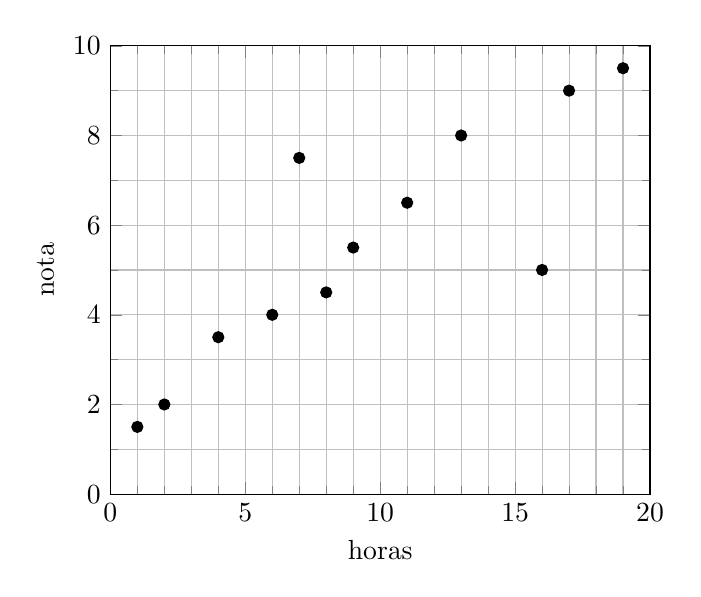
\begin{tikzpicture}
		\begin{axis}[
			grid=both,
			xmin=0, xmax=20,
			ymin=0, ymax=10,
			minor x tick num = 4,
			minor y tick num = 1,
			nodes near coords,
			xlabel=horas,
			ylabel=nota
		]
			
		\addplot+[only marks, point meta=explicit symbolic, mark=*]
			coordinates {
				(1, 1.5)
				(2, 2)
				(4, 3.5)
				(6, 4)
				(8, 4.5)
				(9, 5.5)
				(11, 6.5)
				(13, 8)
				(17, 9)
				(19, 9.5)
				%outliers
				(16, 5)
				(7, 7.5)
		};
		\end{axis}
	\end{tikzpicture}
\end{figure}

Com base nisso, estime a nota dos alunos abaixo utilizando os algoritmos 1NN e 3NN.
\begin{itemize}
	\item Aluno A: 4 horas.
	\item Aluno B: 15 horas.
	\item Aluno C: 7 horas.
	\item Aluno D: 19 horas.
	\item Aluno E: 10 horas.
\end{itemize}
\end{exercise}

\begin{exercise}
Considere o mesmo cenário do exercício anterior e classifique os dados usando o algoritmo de 3NN ponderado pelo inverso do quadrado da distância.
\end{exercise}

\begin{exercise}
Considere o conjunto de dados para determinação da qualidade do vinho disponível em \url{http://archive.ics.uci.edu/ml/datasets/Wine+Quality}. Implemente o algoritmo de $k$NN com diferentes valores de $k$. Trate o problema como classificação e regressão (o conjunto de dados permite isso). Apresente um relatório contendo os resultados obtidos por cada algoritmo, as matrizes de confusão, custo e métricas de avaliação.
\end{exercise}

\begin{exercise}
Modifique a implementação do exercício anterior e utilize alguma das bibliotecas apresentadas na apostila (ou outra da sua escolha) para a execução do algoritmo de $k$NN. Apresente o mesmo relatório com os resultados e compare com a sua implementação.
\end{exercise}

\begin{exercise}
Selecione um conjunto de dados de sua preferência em \url{http://archive.ics.uci.edu/ml/index.php}. Utilize a ferramenta Weka para executar o algoritmo de $k$NN e analise os resultados apresentados pela ferramenta. Compare os resultados para diferentes valores de $k$.
\end{exercise}

\begin{exercise}
Considere a árvore de decisão apresentada abaixo. Esta árvore decide sobre comprar ou não um veículo, com base nas suas características. Utilizando a árvore, classifique os elementos abaixo.

\begin{table}[h]
	\centering
	\begin{tabular}{rllrc}
		\hline
		\textbf{Valor} & \textbf{Consumo} & \textbf{Opcionais} & \textbf{Potência} & \textbf{Comprar?} \\ \hline
		     78.000,00 & Alto             & Sim                &               112 &         ?         \\
		     43.000,00 & Baixo            & Não                &                88 &         ?         \\
		     26.000,00 & Baixo            & Sim                &                82 &         ?         \\
		    112.000,00 & Baixo            & Sim                &               120 &         ?         \\
		     50.000,00 & Alto             & Não                &                96 &         ?         \\ \hline
	\end{tabular}
\end{table}

\begin{figure}[h]
	\centering
	\tikzstyle{no} = [draw, rectangle, inner sep=7pt, minimum width=2.5cm]
	\tikzstyle{folha} = [draw, ellipse, inner sep=5pt, minimum width=2cm, dashed]
	\tikzstyle{texto} = [pos=.5, fill=white]
	
	\begin{tikzpicture}
	\node[no] (valor) at (0,0) {Valor};
	
	\node[no] (consumo) at (-4,-2.5) {Consumo};
	\node[no] (opcionais) at (4,-2.5) {Opcionais};
	
	\node[no] (potencia) at (-2.5,-5) {Potência};
	\node[no] (consumo2) at (2.5,-5) {Consumo};
	
	\node[folha] (sim1) at (-5.5,-5) {Sim};
	\node[folha] (sim2) at (-3.75,-7.5) {Sim};
	\node[folha] (nao1) at (-1.25,-7.5) {Não};
	\node[folha] (sim3) at (1.25,-7.5) {Sim};
	\node[folha] (nao2) at (3.75,-7.5) {Não};
	\node[folha] (sim4) at (5.5,-5) {Sim};
	
	\draw (valor) -- (consumo) node[texto] {\small $\leq 50.000$};
	\draw (valor) -- (opcionais) node[texto] {\small $> 50.000$};
	\draw (opcionais) -- (consumo2) node[texto] {\small Não};
	\draw (consumo) -- (potencia) node[texto] {\small Alto};
	\draw (consumo) -- (sim1) node[texto] {\small Baixo};
	\draw (potencia) -- (sim2) node[texto] {\small $> 90$};
	\draw (potencia) -- (nao1) node[texto] {\small $\leq 90$};
	\draw (consumo2) -- (sim3) node[texto] {\small Baixo};
	\draw (consumo2) -- (nao2) node[texto] {\small Alto};
	\draw (opcionais) -- (sim4) node[texto] {\small Sim};
	
	\end{tikzpicture}
\end{figure}
\end{exercise}

\begin{exercise}
Considere a árvore de decisão apresentada no exercício anterior. Represente-a como (i) um conjunto de regras na estrutura \texttt{se-então} e (ii) uma conjunção de disjunções.
\end{exercise}

\begin{exercise}
Considere o conjunto de dados sobre \textit{jogar tênis} (tabela abaixo). Calcule a entropia e o ganho de informação e indique qual o melhor atributo para compor a raiz da árvore de decisão.

\insertspace

\begin{table}[h]
	\centering
	\def\arraystretch{1.3}
	\begin{tabular}{ccccc}
		\hline
		\textbf{Clima} & \textbf{Temperatura} & \textbf{Umidade} & \textbf{Vento} & \textbf{Jogar?} \\ \hline
		  ensolarado   &        quente        &       alta       &     falso      &       não       \\
		  ensolarado   &        quente        &       alta       &   verdadeiro   &       não       \\
		   nublado     &        quente        &       alta       &     falso      &       sim       \\
		   chuvoso     &        amena         &       alta       &     falso      &       sim       \\
		   chuvoso     &         fria         &      normal      &     falso      &       sim       \\
		   chuvoso     &         fria         &      normal      &   verdadeiro   &       não       \\
		   nublado     &         fria         &      normal      &   verdadeiro   &       sim       \\
		  ensolarado   &        amena         &       alta       &     falso      &       não       \\
		  ensolarado   &         fria         &      normal      &     falso      &       sim       \\
		   chuvoso     &        amena         &      normal      &     falso      &       sim       \\
		  ensolarado   &        amena         &      normal      &   verdadeiro   &       sim       \\
		   nublado     &        amena         &       alta       &   verdadeiro   &       sim       \\
		   nublado     &        quente        &      normal      &     falso      &       sim       \\
		   chuvoso     &        amena         &       alta       &   verdadeiro   &       não       \\ \hline
	\end{tabular}
\end{table}
\end{exercise}

\begin{exercise}
Com base na árvore de decisão apresentada na Figura~\ref{fig:exemplo-arvore-decisao} da Seção~\ref{sec:arvores-decisao-esquema-geral}, calcule a qualidade do modelo utilizando para teste os dados do exercício anterior. Mostre a matriz de confusão, a acurácia e a taxa de erro. Com base na matriz de custo abaixo, calcule o custo deste modelo.

\begin{table}[h]
	\centering
	\begin{tabular}{cc|c|c|}
		\cline{3-4}
		&                   & \multicolumn{2}{c|}{\textbf{Classe prevista}} \\ \cline{3-4} 
		&                   & \textbf{Jogar}     & \textbf{Não jogar}     \\ \hline
		\multicolumn{1}{|c|}{\multirow{2}{*}{\textbf{Classe real}}} & \textbf{Jogar} & -10           & 15           \\ \cline{2-4} 
		\multicolumn{1}{|c|}{}                                      & \textbf{Não jogar} & 50           & -10           \\ \hline
	\end{tabular}
\end{table}

\end{exercise}

\begin{exercise}
Apresente a árvore de decisão completa para o problema de \textit{jogar tênis}.
\end{exercise}

\begin{exercise}
Considere o conjunto de dados disponível em \url{https://goo.gl/1H215P}. Estes dados apresentam informações sobre um experimento realizado com 30 voluntários com idades entre 19 e 48 anos. Neste experimento os usuários realizaram diferentes atividades com seus smartphones (caminhada, subida e descida de escadas, etc.). Foram capturados dados a partir dos sensores de giroscópio e acelerômetro. A tarefa consiste em determinar a atividade que o usuário está realizando, com base nos dados obtidos pelos sensores. Utilize a ferramenta Weka para induzir uma árvore de decisão para realização desta tarefa. Mostre a árvore induzida e seu desempenho nos testes.
\end{exercise}

\begin{exercise}
Modifique o exercício anterior, substituindo o Weka por uma biblioteca de \textit{machine learning} (recomenda-se o uso da biblioteca JavaML). Mostre os resultados obtidos utilizando a biblioteca e compare com a avaliação obtida no exercício anterior.
\end{exercise}